\documentclass[border=4pt]{standalone}
\usepackage{fontspec}
\usepackage{amsmath}
\usepackage{unicode-math}
\setmainfont{Latin Modern Roman}
\setmathfont{Latin Modern Math}
\usepackage{pgfplots}
\usepackage{pgfplotstable}
\pgfplotsset{compat=1.18}
\usepackage{tkz-euclide}
\usetikzlibrary{arrows.meta,calc,angles,quotes,patterns,3d,backgrounds}
\definecolor{ink}{HTML}{123428}
\definecolor{asy}{HTML}{475569}
\definecolor{mint}{HTML}{86e0bd}
\tikzset{asym/.style={asy, line width=0.9pt, dash pattern=on 5pt off 3.5pt},
         guide/.style={gray!70, line width=0.6pt, densely dotted},
         dot/.style={circle, inner sep=0pt, minimum size=5pt, draw=white, line width=0.5pt},
         odot/.style={circle, inner sep=0pt, minimum size=5.5pt, fill=white, line width=1pt},
         lab/.style={font=\footnotesize, inner sep=1.5pt, text=ink}}
\begin{document}
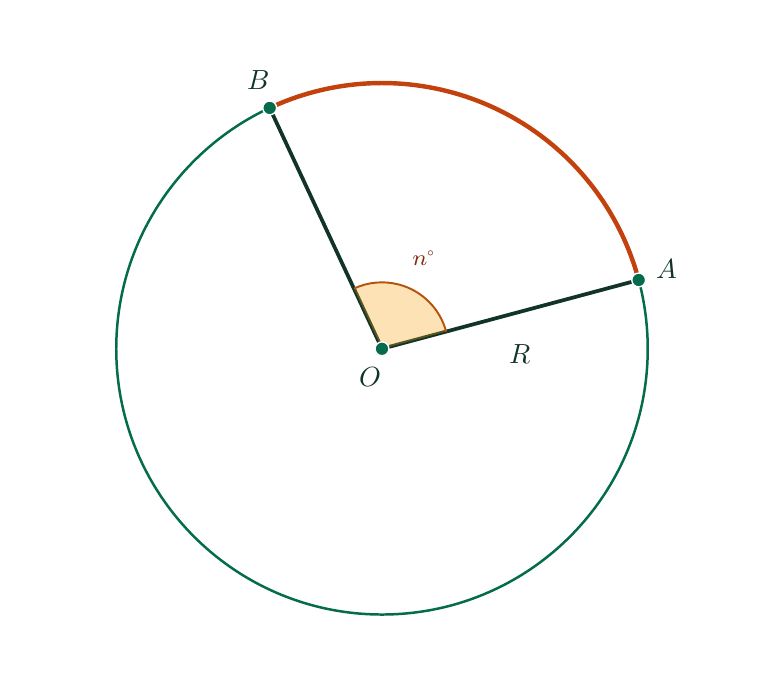
\begin{tikzpicture}[x=1.4062cm, y=1.4062cm]
\tkzDefPoint(0,0){O}
\tkzDefPoint(2.3182,0.6212){A}
\tkzDefPoint(-1.0143,2.1751){B}
\tkzDefPoint(2.4,0){tmp1}
\begin{scope}
\clip (-3.2,-2.9) rectangle (3.2,2.9);
\tkzDrawCircle[draw={rgb,255:red,4;green,107;blue,77}, line width=0.9pt](O,tmp1)
\tkzDrawSegment[draw=ink, line width=1.35pt](O,A)
\tkzDrawSegment[draw=ink, line width=1.35pt](O,B)
\draw[draw={rgb,255:red,194;green,65;blue,12}, line width=1.6pt] (2.3182,0.6212) arc[start angle=15.0009, end angle=115.0007, radius=3.37498cm];
\end{scope}
\tkzFillAngle[size=0.6, fill={rgb,255:red,245;green,158;blue,11}, fill opacity=0.3](A,O,B)
\tkzMarkAngle[size=0.6, draw={rgb,255:red,180;green,83;blue,9}, line width=0.7pt, mark=none](A,O,B)
\tkzLabelAngle[pos=0.899, text={rgb,255:red,124;green,45;blue,18}, font=\footnotesize](A,O,B){$n^\circ$}
\node[dot, fill={rgb,255:red,4;green,107;blue,77}] at (O) {};
\node[dot, fill={rgb,255:red,4;green,107;blue,77}] at (A) {};
\node[dot, fill={rgb,255:red,4;green,107;blue,77}] at (B) {};
\node[lab, font=\normalsize] at (1.25,-0.05) {$R$};
\node[lab, font=\normalsize, anchor=center, xshift=-4.21pt, yshift=-10.16pt] at (0,0) {$O$};
\node[lab, font=\normalsize, anchor=center, xshift=10.16pt, yshift=4.21pt] at (2.3182,0.6212) {$A$};
\node[lab, font=\normalsize, anchor=center, xshift=-4.21pt, yshift=10.16pt] at (-1.0143,2.1751) {$B$};
\end{tikzpicture}
\end{document}
